\section{Вычислительные эксперименты}

    \subsection{Алгоритм}
        Для реализации моделей сделаем замену переменных \( \beta(t) = \dot{\alpha}(t) \), и получим систему дифференциальных уравнений первого порядка:
        \[
            \begin{cases}
                & \dot{\beta} + w^2 \sin \alpha = 0, \\
                & \beta = \dot{\alpha}, \\
                & \beta(0) = \alpha_1, \quad \alpha(0) = \alpha_0.
            \end{cases} \Rightarrow
            \begin{cases}
                & \dot{\beta} = - w^2 \sin \alpha, \\
                & \dot{\alpha} = \beta, \\
                & \beta(0) = \alpha_1, \quad \alpha(0) = \alpha_0.
            \end{cases}
        \]
        Для системы данного вида можно применять различные численные методы. Уравнения с дополнительными силами аналогично приводятся к такому виду.

        Для компьютерного вычисления будем использовать метод Рунге-Кутты, с помощью которого получим численное решение системы дифференциальных уравнений с заданными параметрами. После чего построим их решения и фазовые плоскости.

        Для модели с силой трения и вынуждающими колебаниями для каждой частоты колебаний найдём максимальную амплитуду, после того как установится равновесие сил.


    \subsection{Программа}
        Для расчётов и визуализации был использован язык Python с библиотеками numpy и matplotlib.

        \lstinputlisting[language=Python,
        captionpos=t,
        style=colored,
        basicstyle=\footnotesize\dejavu,
        frame=lines]{src/3model.py}

    \subsection{Результаты}
        Будем строить изменение угла во времени и фазовый портрет системы.
        \subsubsection{Модель без дополнительных сил}
            Сравним линейное и нелинейное дифференциальное уравнение при различных начальных углах наклона и нулевой начальной скорости.

            \begin{figure}[H]
                \centering
                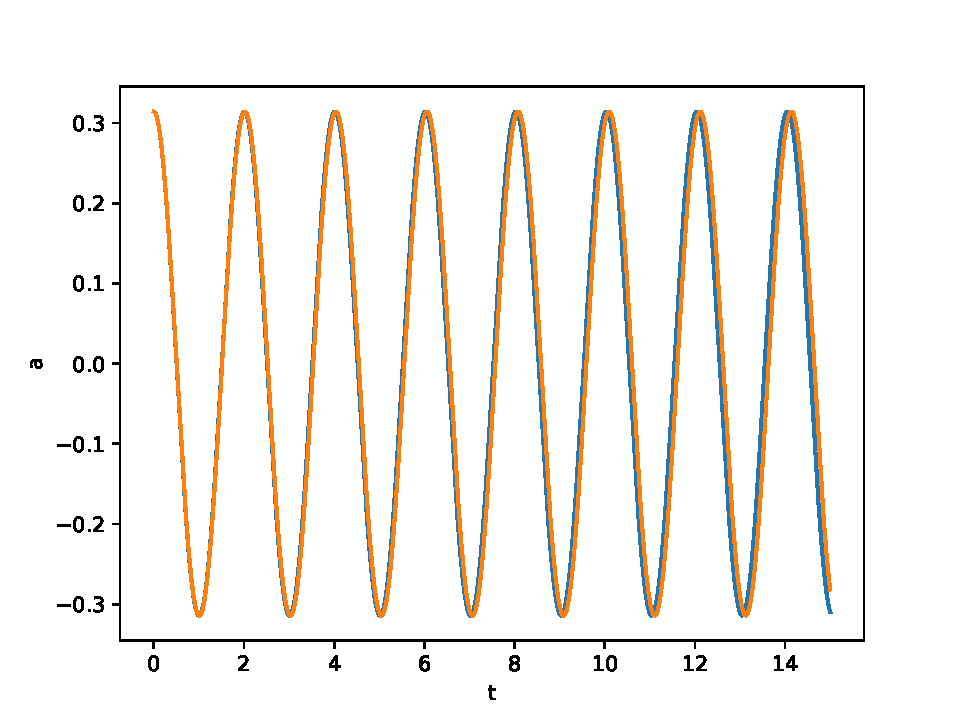
\includegraphics[width=8cm]{pictures/12resonance10.pdf}
                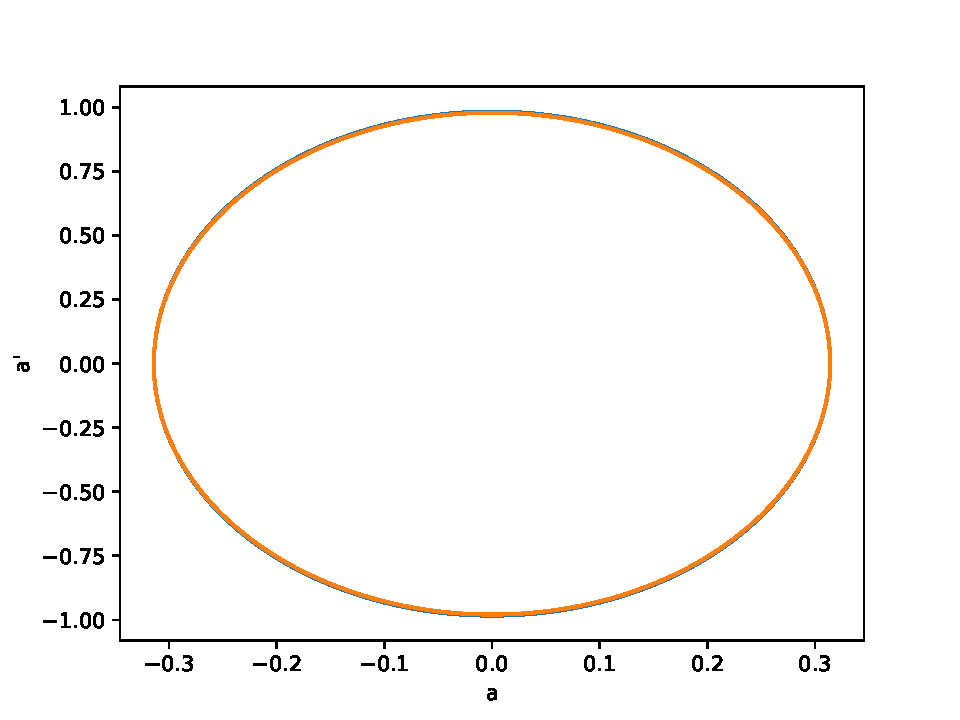
\includegraphics[width=8cm]{pictures/12resonance10p.pdf}
                \caption{$\alpha(0) = \frac{\pi}{10}$.}
            \end{figure}

            \begin{figure}[H]
                \centering
                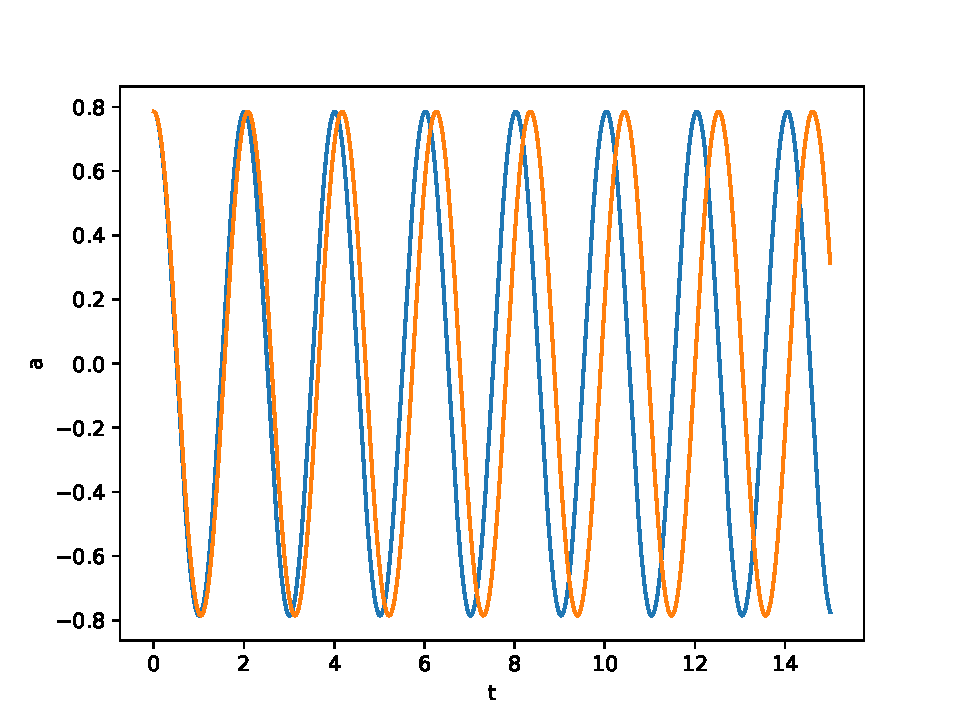
\includegraphics[width=8cm]{pictures/12resonance4.pdf}
                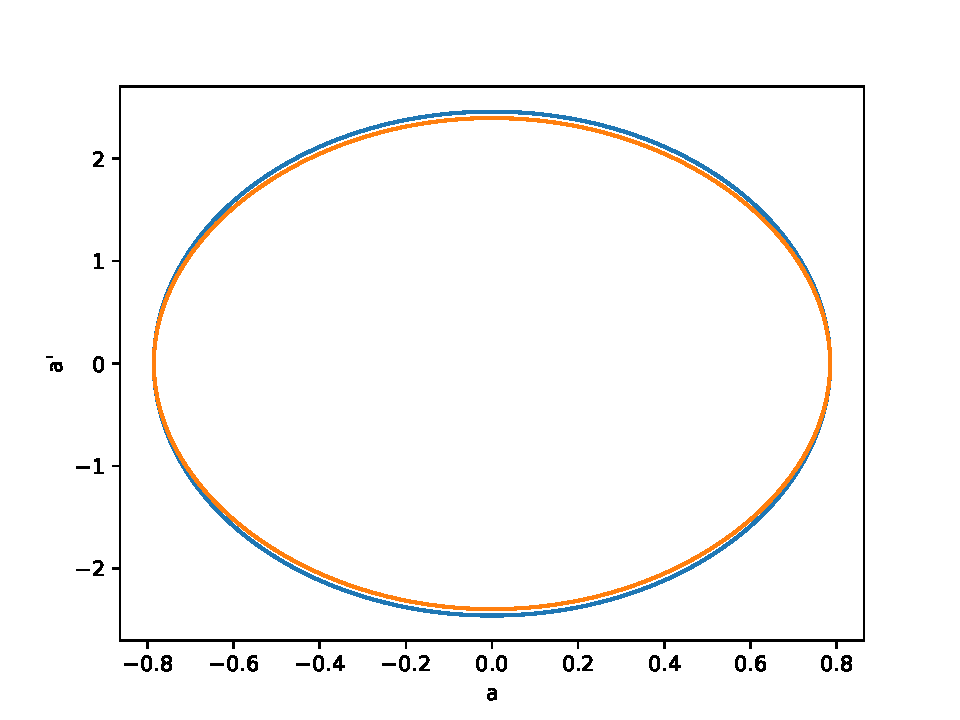
\includegraphics[width=8cm]{pictures/12resonance4p.pdf}
                \caption{$\alpha(0) = \frac{\pi}{4}$.}
            \end{figure}

            Синей кривой визуализирована линейная модель, оранжевой -- нелинейная.
            
            На данных результатах видно, что при небольшом угле наклона разница небольшая, а при большем -- увеличивается период и вместе с этим растёт и погрешность линейной модели. На фазовой плоскости можно увидеть более суженный эллипс у нелинейной модели, что означает меньшую скорость.

        \subsubsection{Модель с трением}
            Рассмотрим результаты влияния трения на маятник.
            \begin{figure}[H]
                \centering
                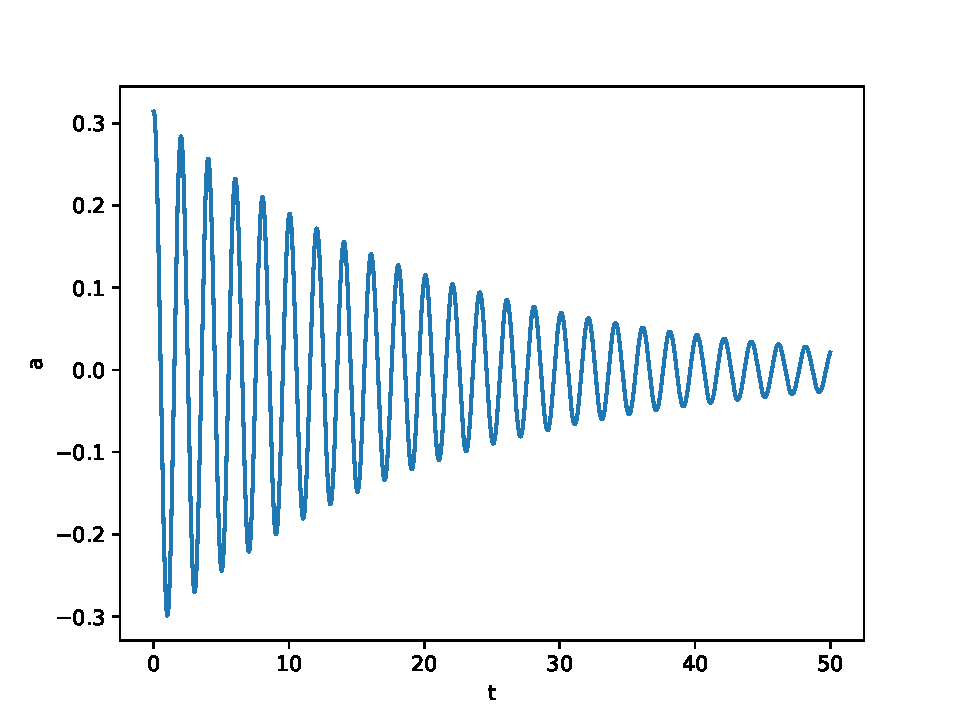
\includegraphics[width=8cm]{pictures/3resonance1.pdf}
                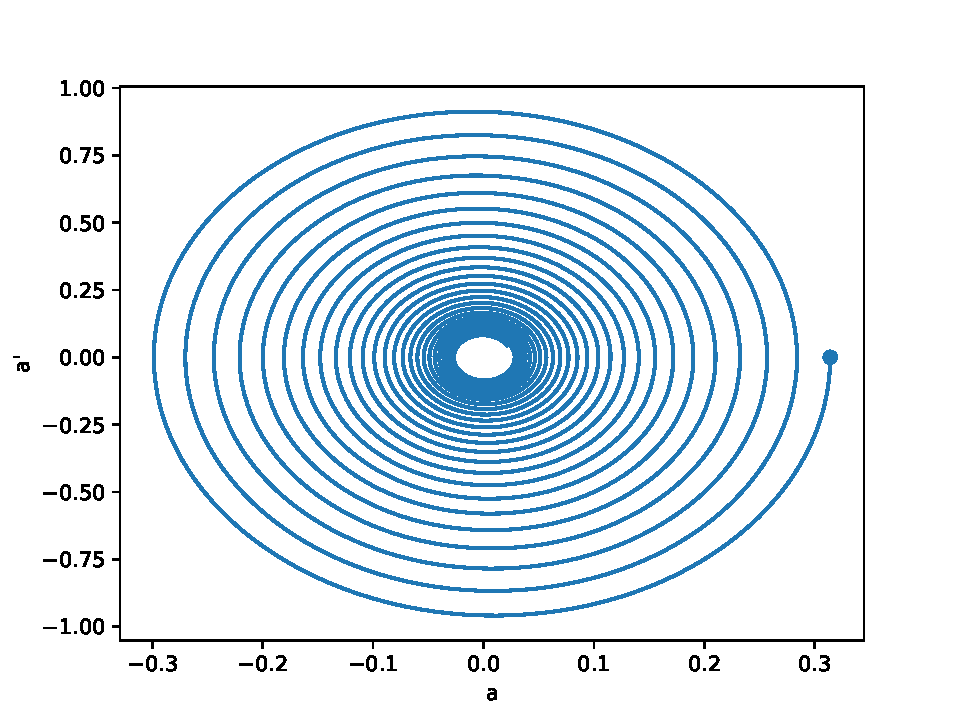
\includegraphics[width=8cm]{pictures/3resonance1p.pdf}
                \caption{$\alpha(0) = \frac{\pi}{10}, \quad \dot{\alpha}(0) = 0, \quad k = 0.1$.}
            \end{figure}
            \begin{figure}[H]
                \centering
                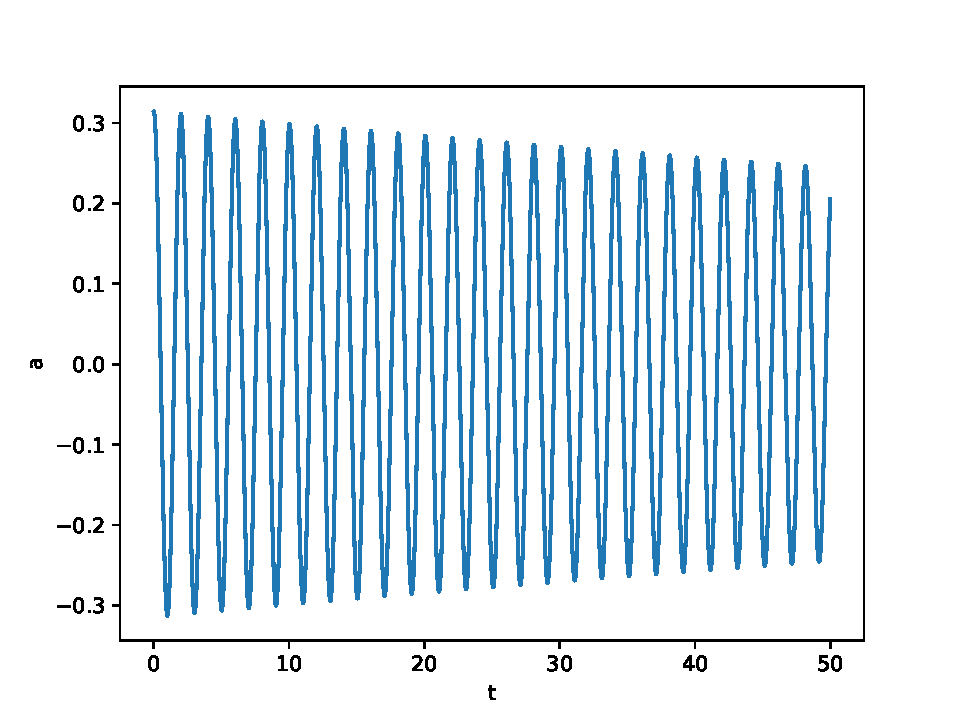
\includegraphics[width=8cm]{pictures/3resonance2.pdf}
                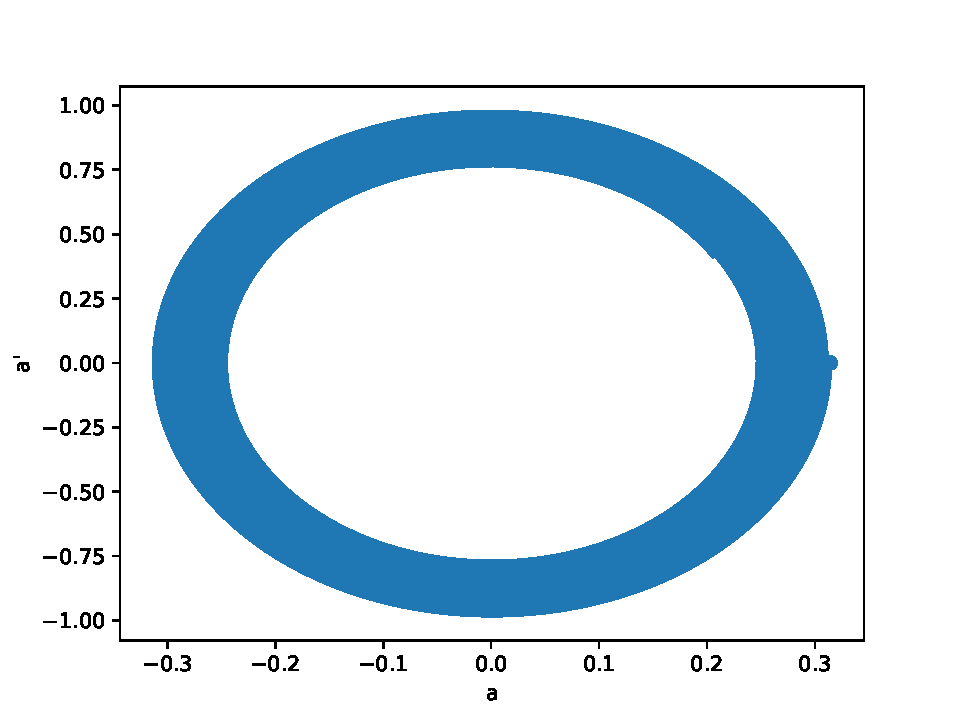
\includegraphics[width=8cm]{pictures/3resonance2p.pdf}
                \caption{$\alpha(0) = \frac{\pi}{10}, \quad \dot{\alpha}(0) = 0, \quad k = 0.01$.}
            \end{figure}

            Видно, что амплитуда колебаний из-за трения со временем уменьшается, поэтому колебания являются затухающими. Кривая на фазовой плоскости из-за затухания постепенно приближается к нулю.

        \subsubsection{Модель с вынуждающими колебаниями}
            Рассмотрим результаты при действии вынуждающих колебаний на маятник с начальными условиями $\alpha(0) = \frac{\pi}{10}, \quad \dot{\alpha}(0) = 0$.
            \begin{figure}[H]
                \centering
                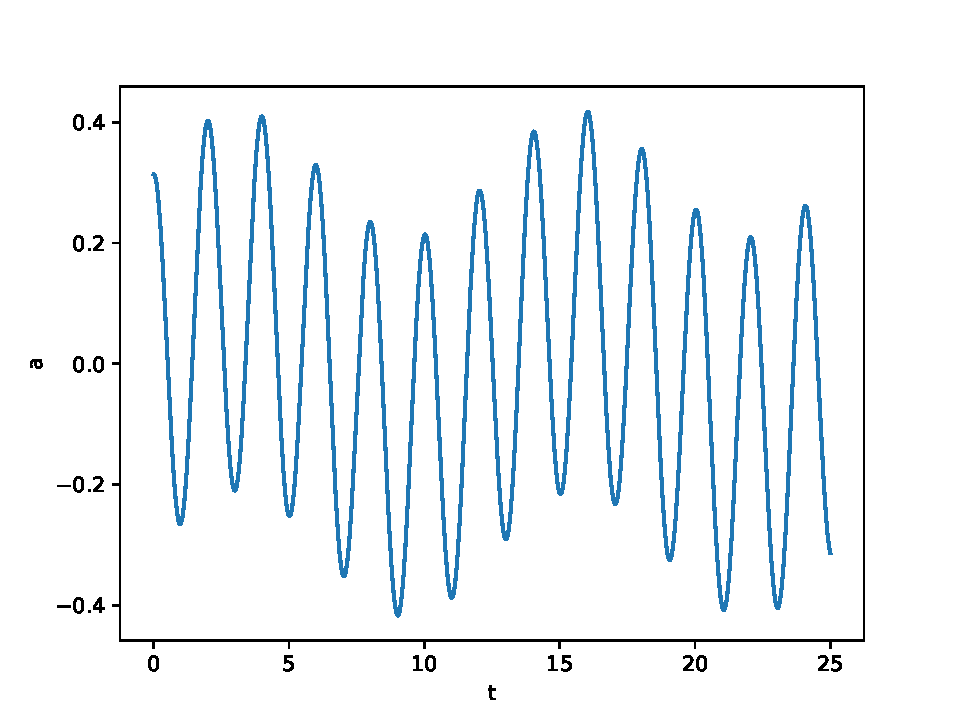
\includegraphics[width=8cm]{pictures/4resonance1.pdf}
                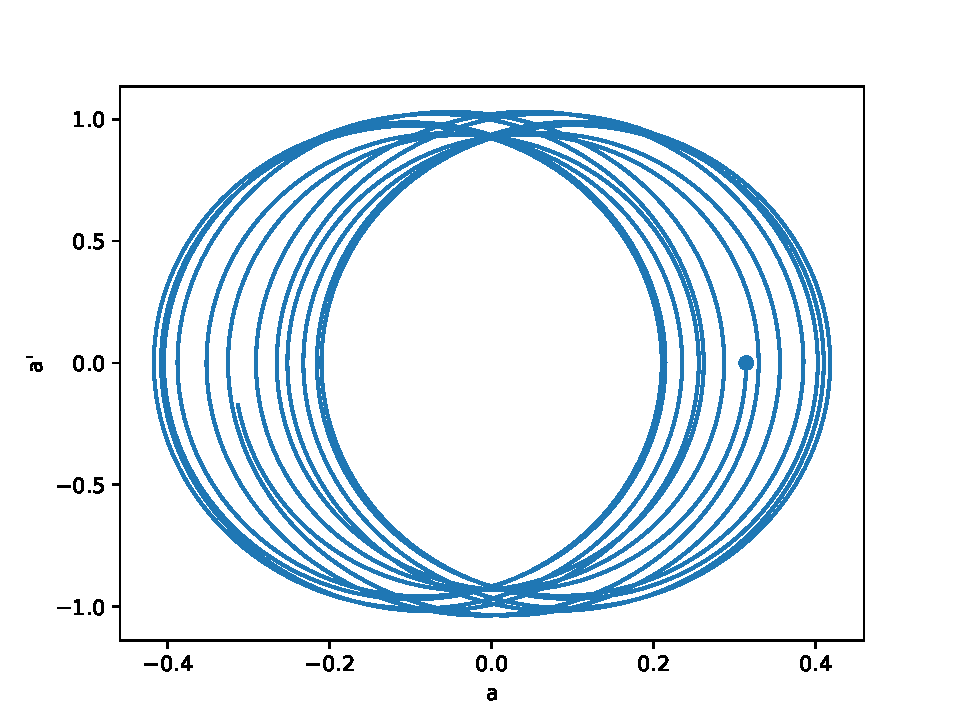
\includegraphics[width=8cm]{pictures/4resonance1p.pdf}
                \caption{$A_f = 1 \quad w_f = 0.5$.}
            \end{figure}

            \begin{figure}[H]
                \centering
                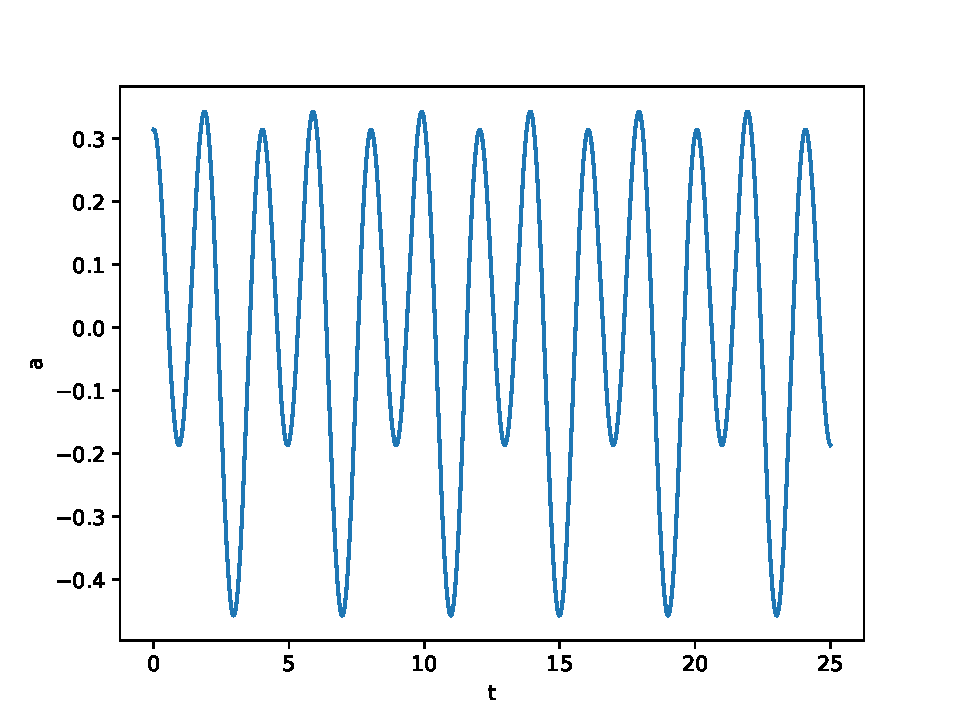
\includegraphics[width=8cm]{pictures/4resonance2.pdf}
                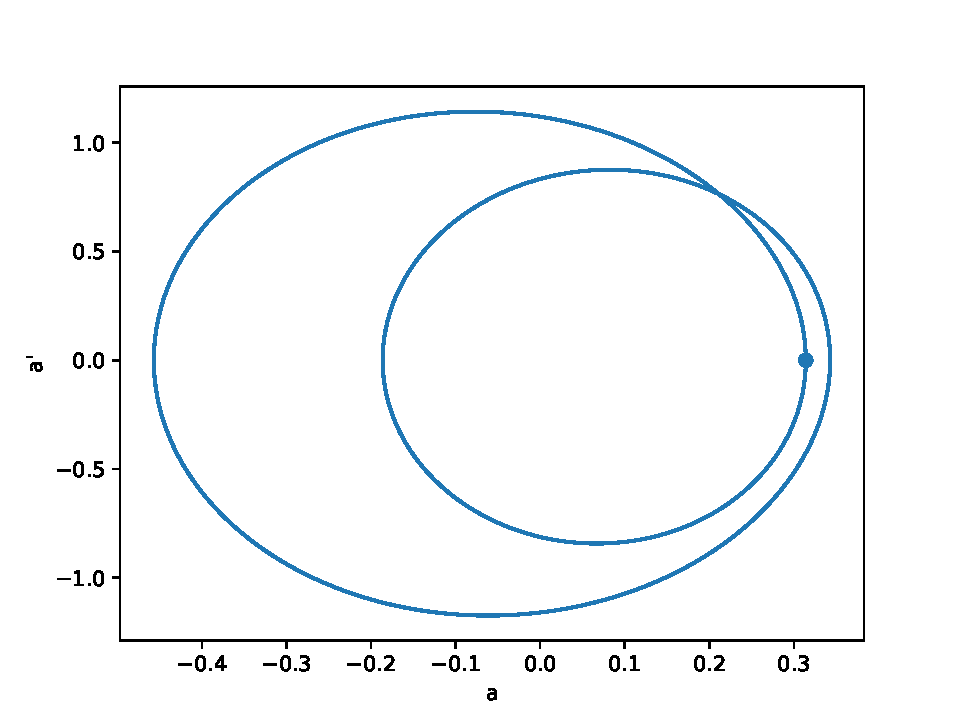
\includegraphics[width=8cm]{pictures/4resonance2p.pdf}
                \caption{$A_f = 1 \quad w_f = \frac{w}{2}$.}
            \end{figure}

            \begin{figure}[H]
                \centering
                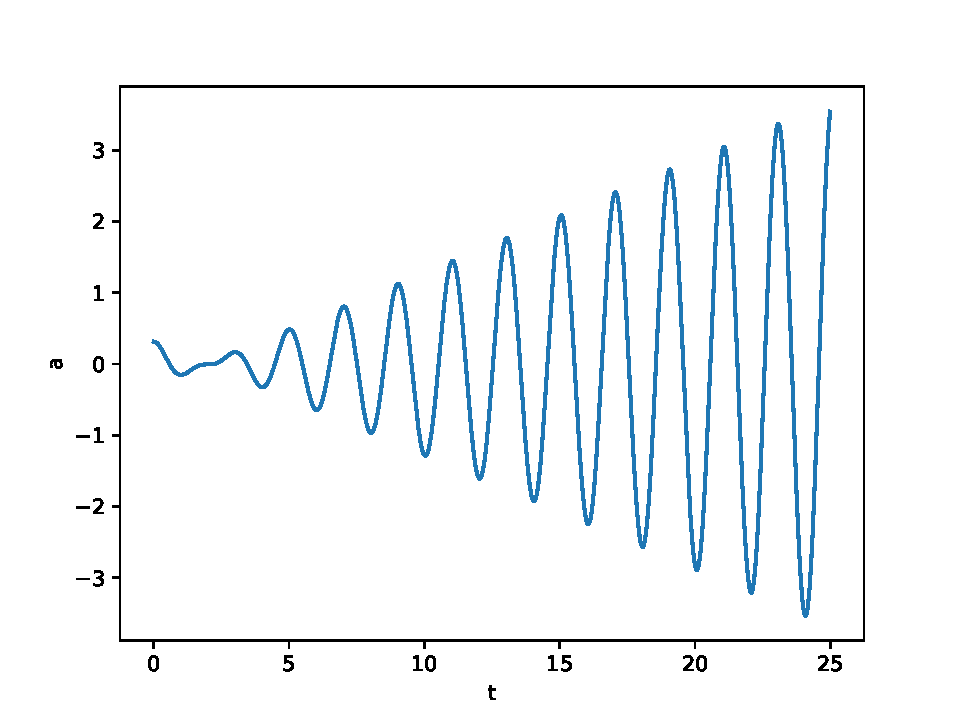
\includegraphics[width=8cm]{pictures/4resonance3.pdf}
                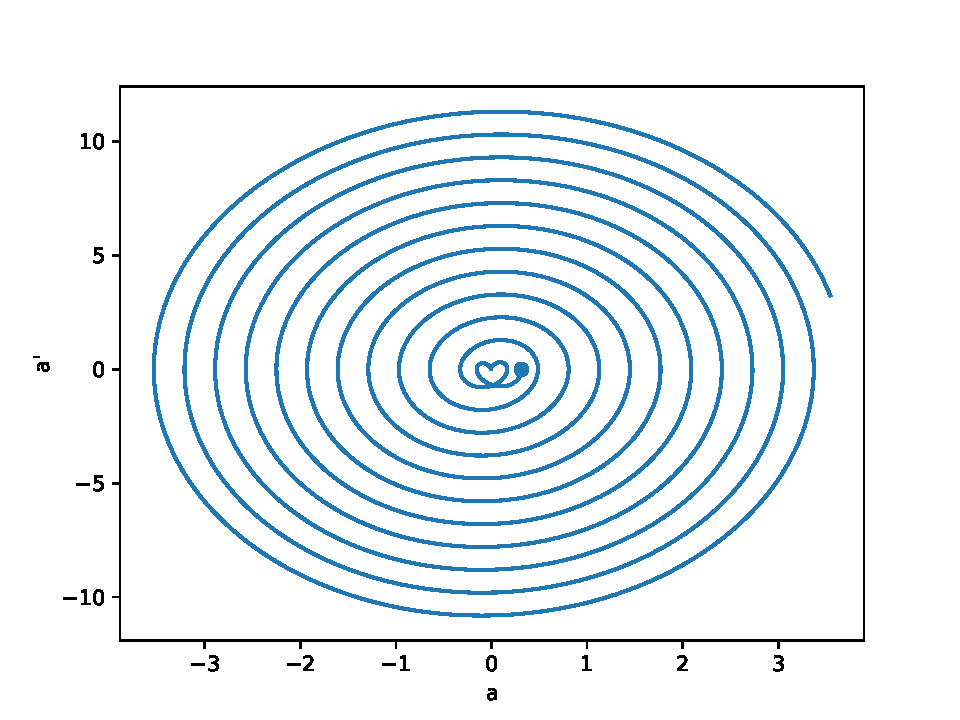
\includegraphics[width=8cm]{pictures/4resonance3p.pdf}
                \caption{$A_f = 1 \quad w_f = w$.}
            \end{figure}
            Резонанс

        \subsubsection{Модель с трением и вынуждающими колебаниями}
            $\alpha(0) = \frac{\pi}{10}, \quad \dot{\alpha}(0) = 0$.
            \begin{figure}[H]
                \centering
                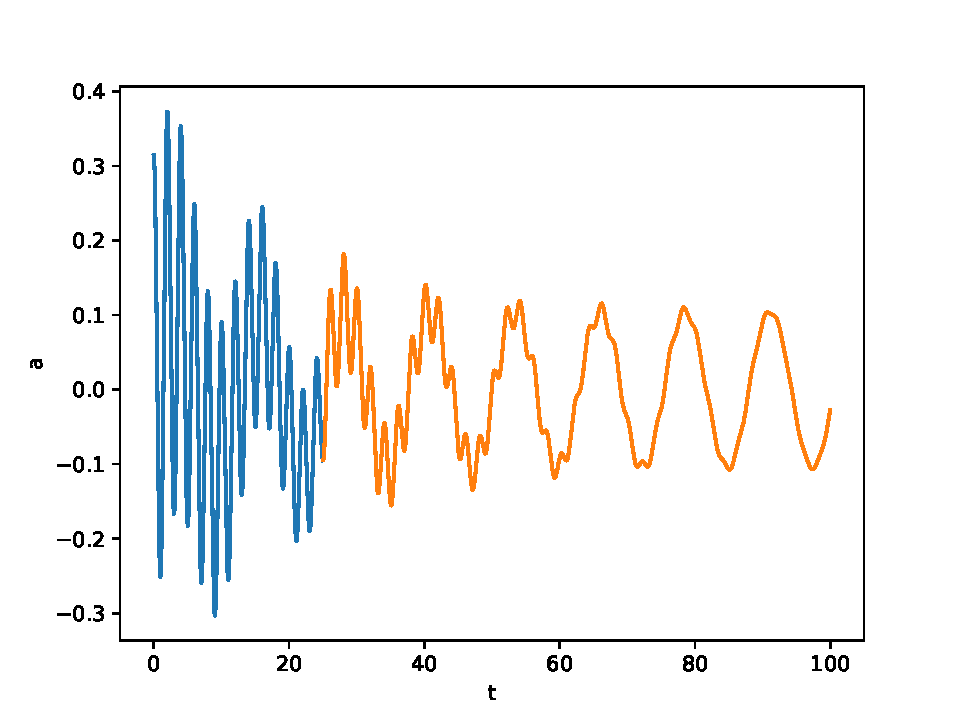
\includegraphics[width=8cm]{pictures/5resonance1.pdf}
                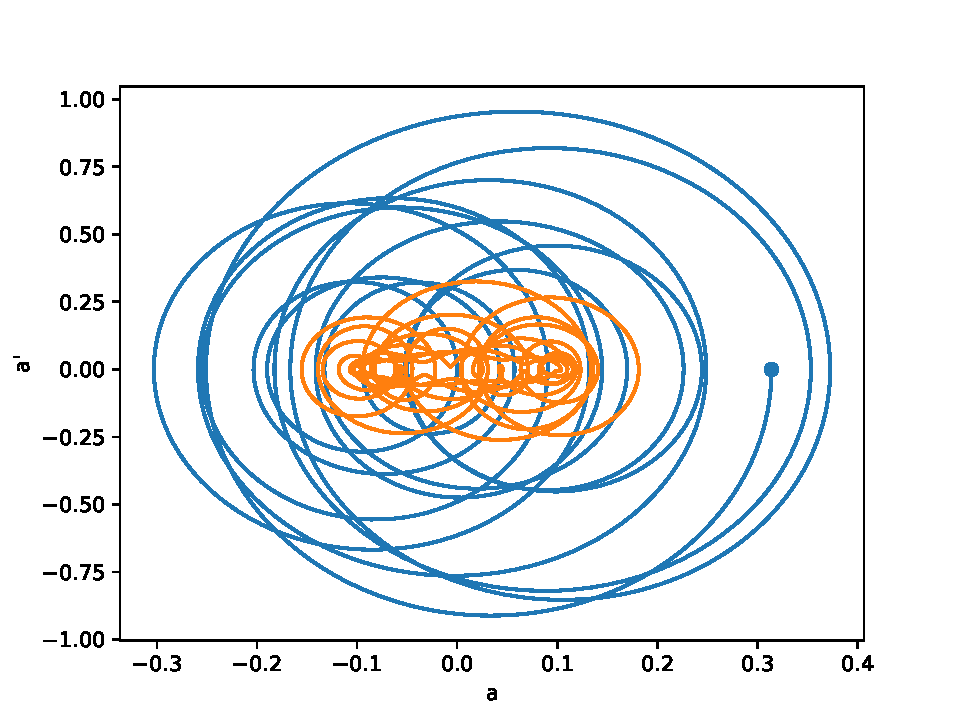
\includegraphics[width=8cm]{pictures/5resonance1p.pdf}
                \caption{$A_f = 1 \quad w_f = 0.5$.}
            \end{figure}

            \begin{figure}[H]
                \centering
                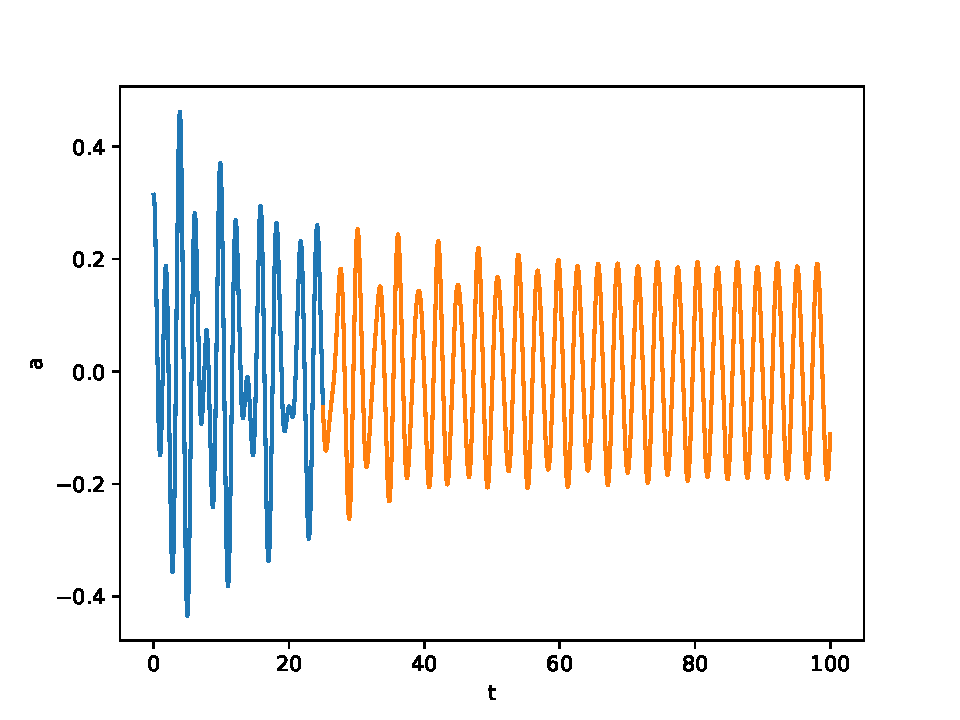
\includegraphics[width=8cm]{pictures/5resonance2.pdf}
                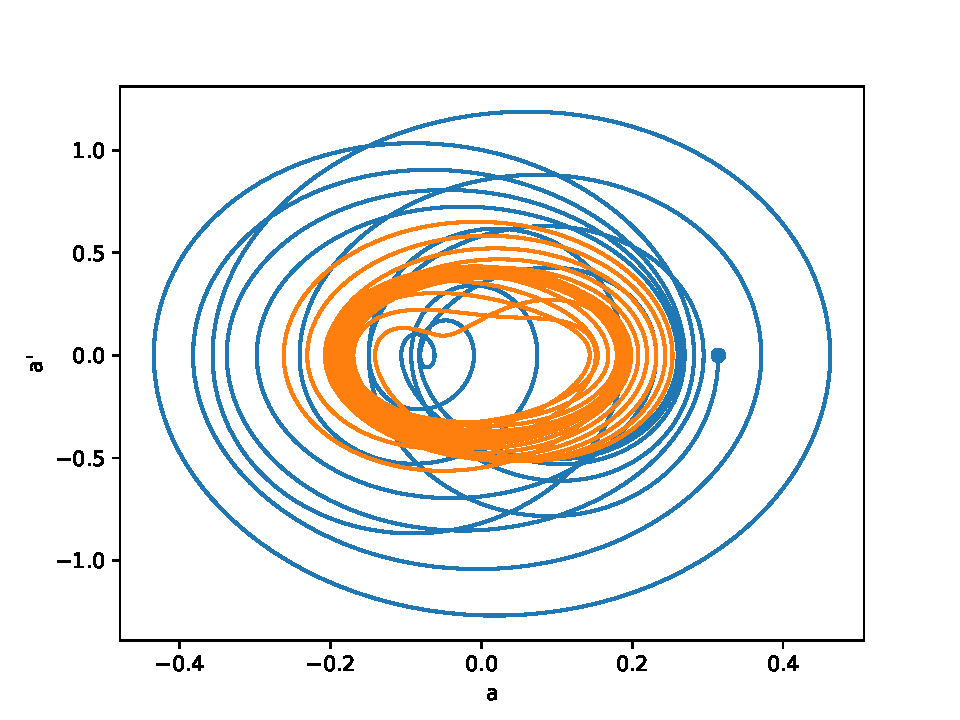
\includegraphics[width=8cm]{pictures/5resonance2p.pdf}
                \caption{$A_f = 1 \quad w_f = w-1$.}
            \end{figure}

            \begin{figure}[H]
                \centering
                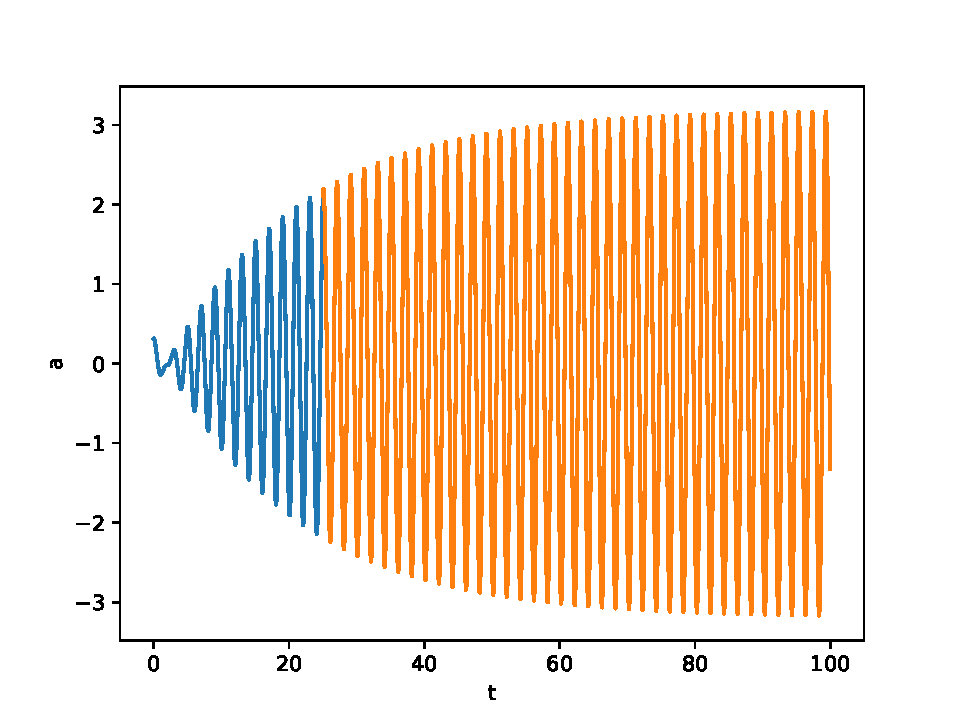
\includegraphics[width=8cm]{pictures/5resonance3.pdf}
                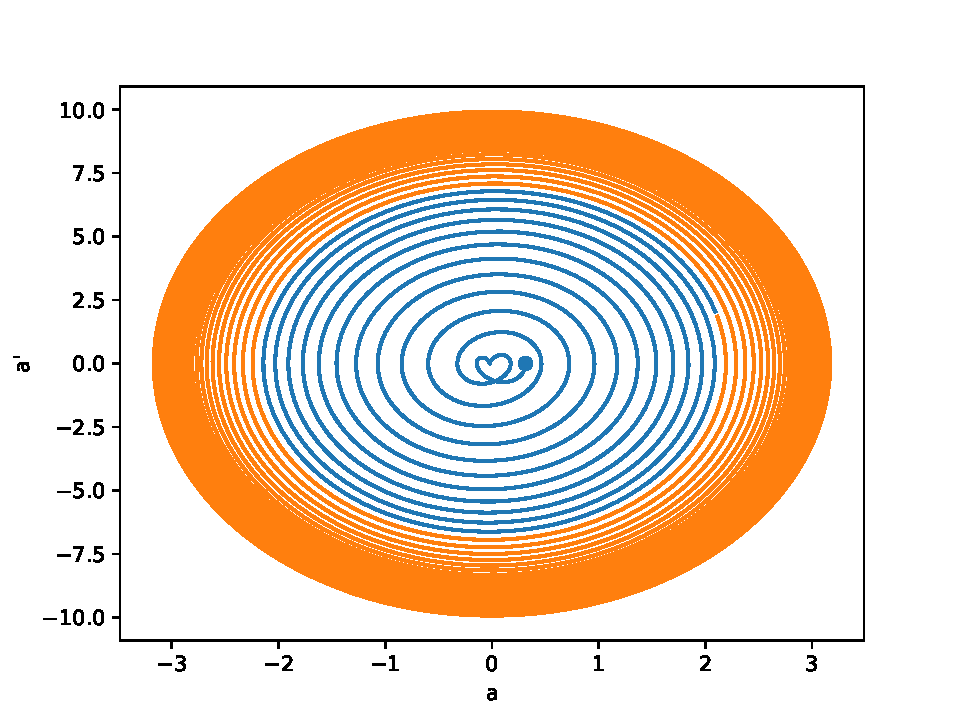
\includegraphics[width=8cm]{pictures/5resonance3p.pdf}
                \caption{$A_f = 1 \quad w_f = w$.}
            \end{figure}

            Резонанс
            \begin{figure}[H]
                \centering
                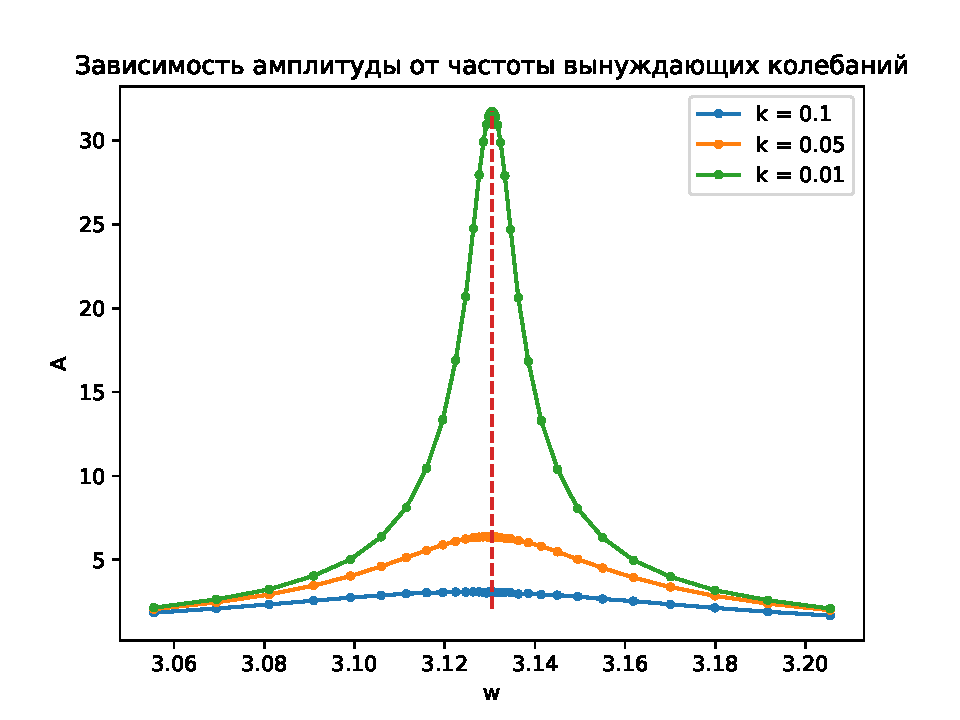
\includegraphics[width=15cm]{pictures/6resonance2.pdf}
            \end{figure}